%! TEX root = ../main.tex
\documentclass[../main.tex]{subfiles}

\begin{document}

\subsection{Fenditura $\qty{0.04}{\mm}$}

Per la fenditura da $\qty{0.04}{\mm}$ ed apertura del sensore pari a $\qty{1.5}{\mm}$ sono stati raccolti $3$ set di dati che sono riportati in \autoref{fig:single scatter 0.04}.

\begin{figure}[ht!]
    \centering
    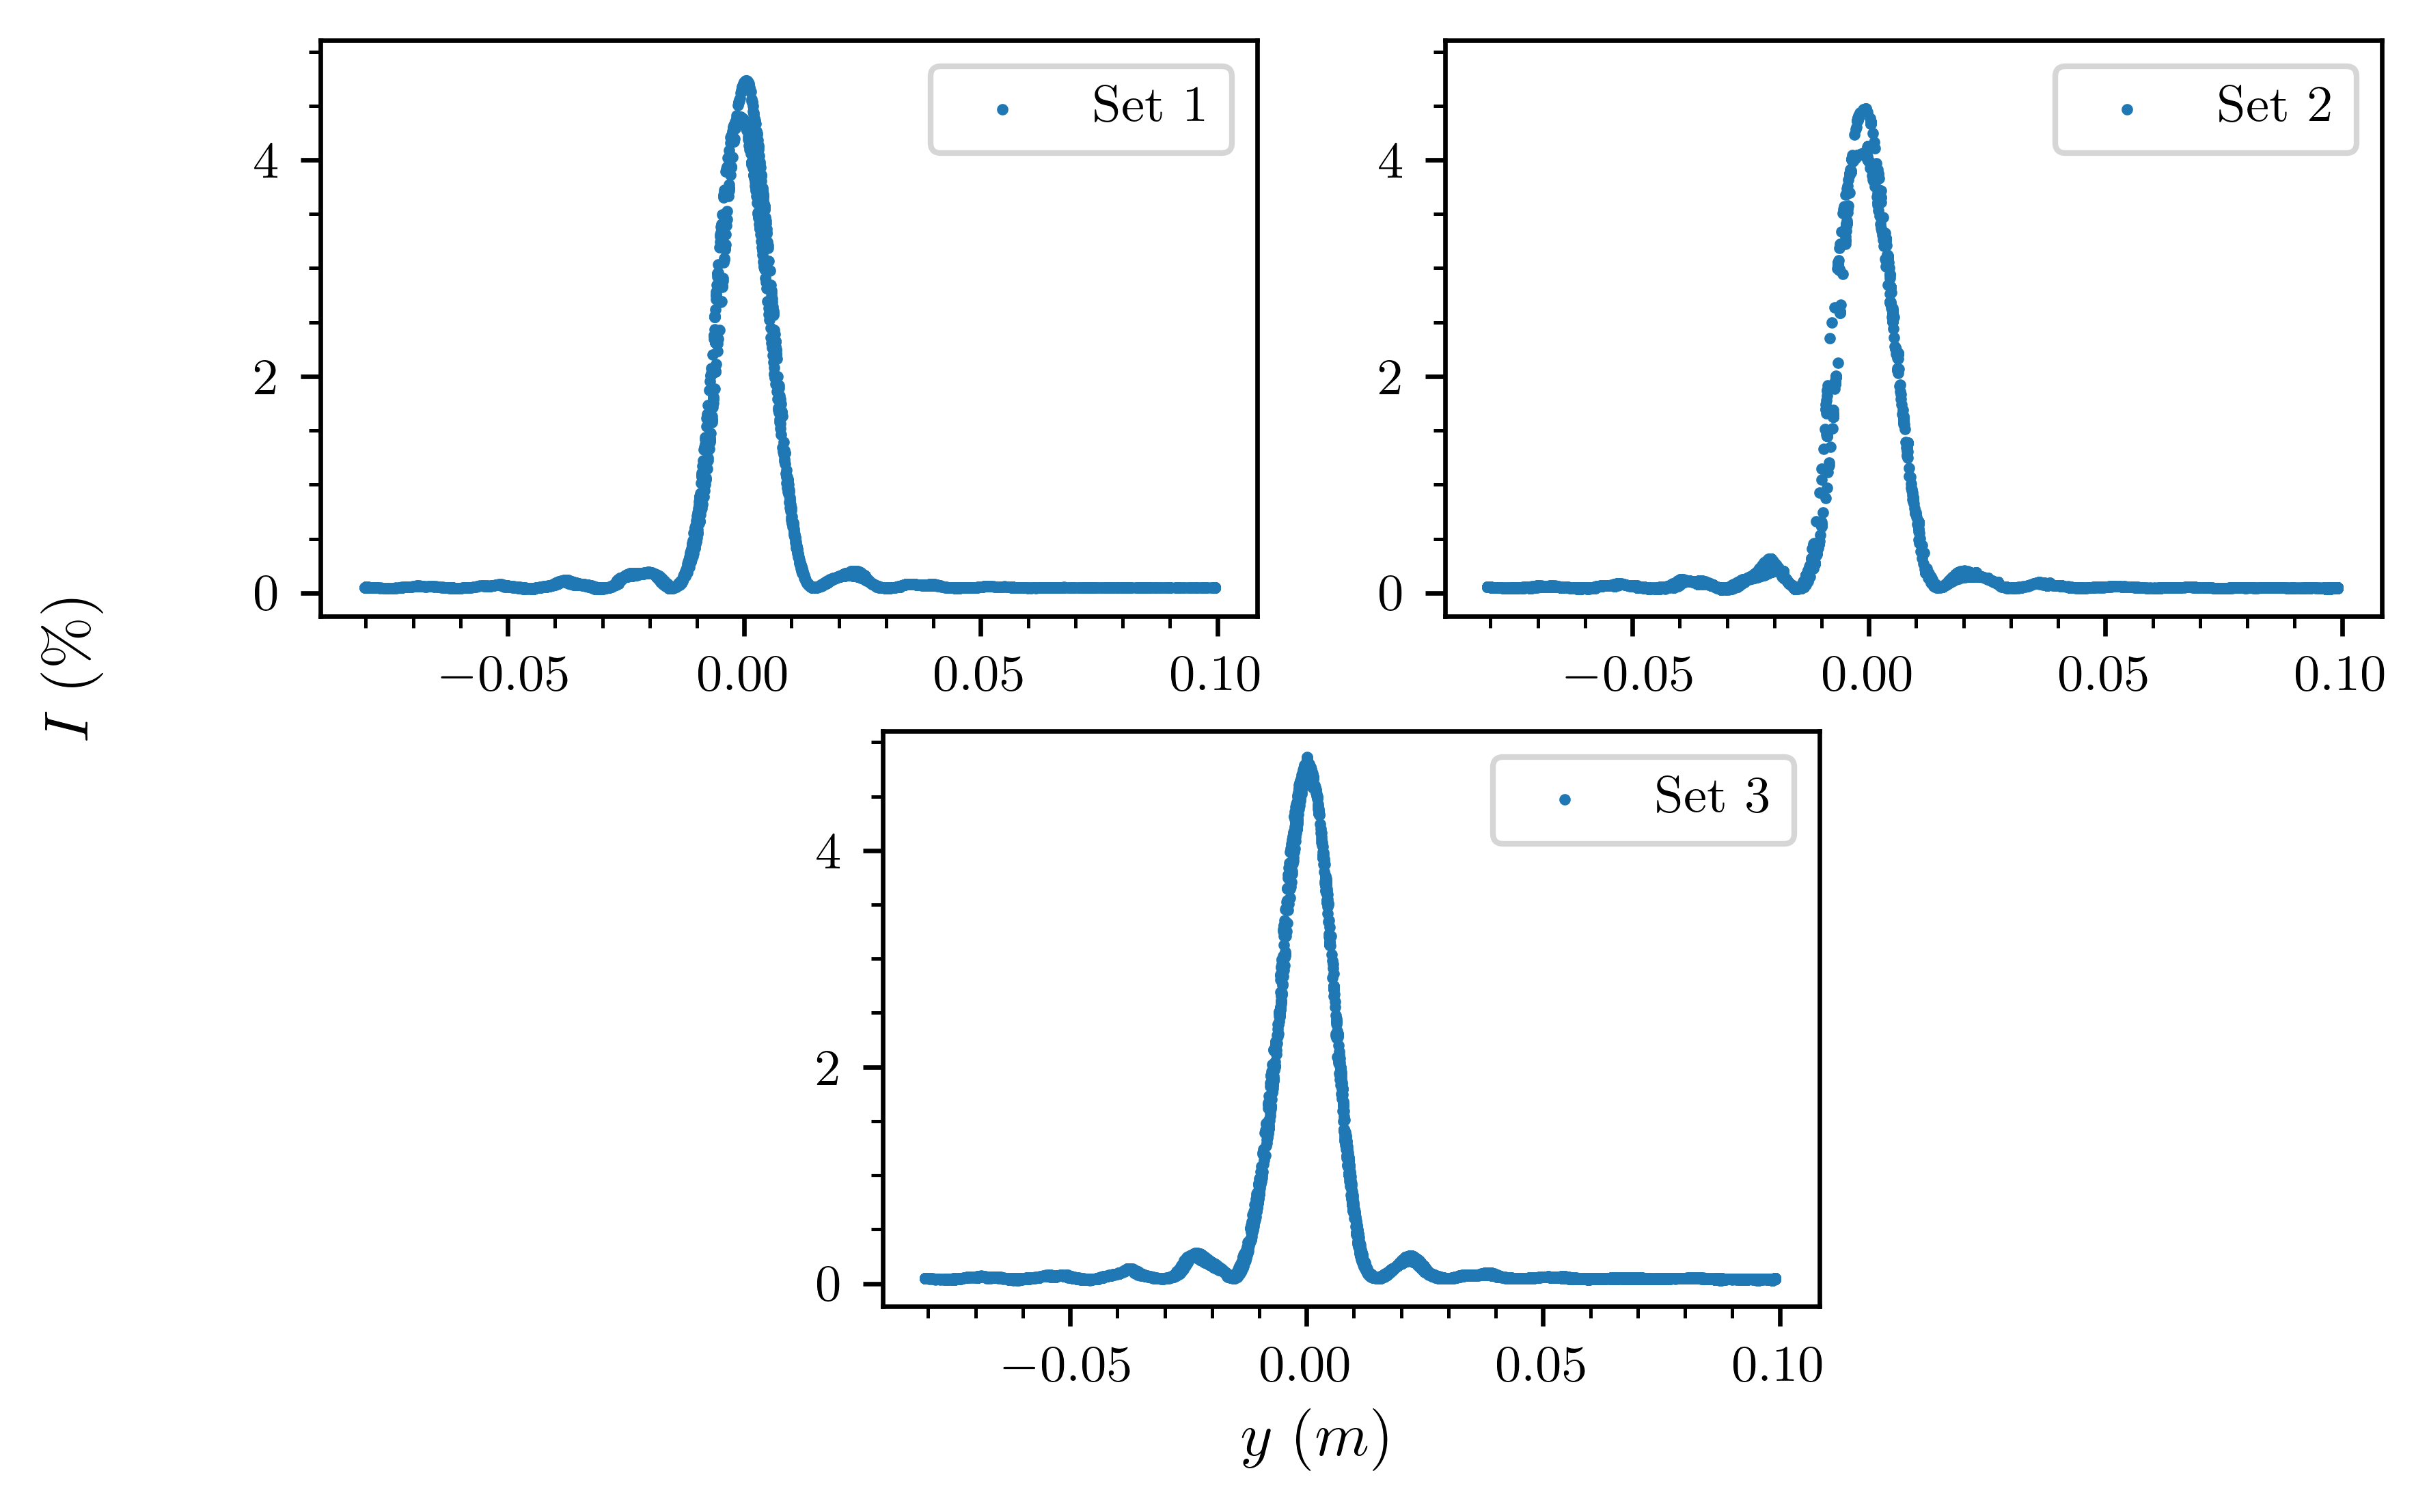
\includegraphics{single_scatter_0.04.png}
    \caption{Misure dell'intensità luminosa $I$ in funzione della posizione $y$ (in metri) del sensore con apertura pari a \qty{1.5}{\mm} e fenditura di \qty{0.04}{\mm}. Le curve presentano un picco centrale con una leggera variazione di intensità tra l'andata e il ritorno del sensore, maggiormente evidente nei set $1$ e $2$. La forma dei massimi laterali differisce tra i vari set.}
    \label{fig:single scatter 0.04}
\end{figure}

Sovrapponendo i set si è proceduto ad individuare la posizione dei minimi attribuendogli una barra d'errore sufficientemente grande da rendere la misura compatibile con tutti i set. Le posizioni dei minimi ottenute dalla \autoref{fig:minimi 0.04} sono riportate in \autoref{tab:minimi 0.04} di fianco ai valori della fenditura ricavati utilizzando l'\autoref{eq:y=0 values}.

\begin{figure}[ht!]
    \centering
    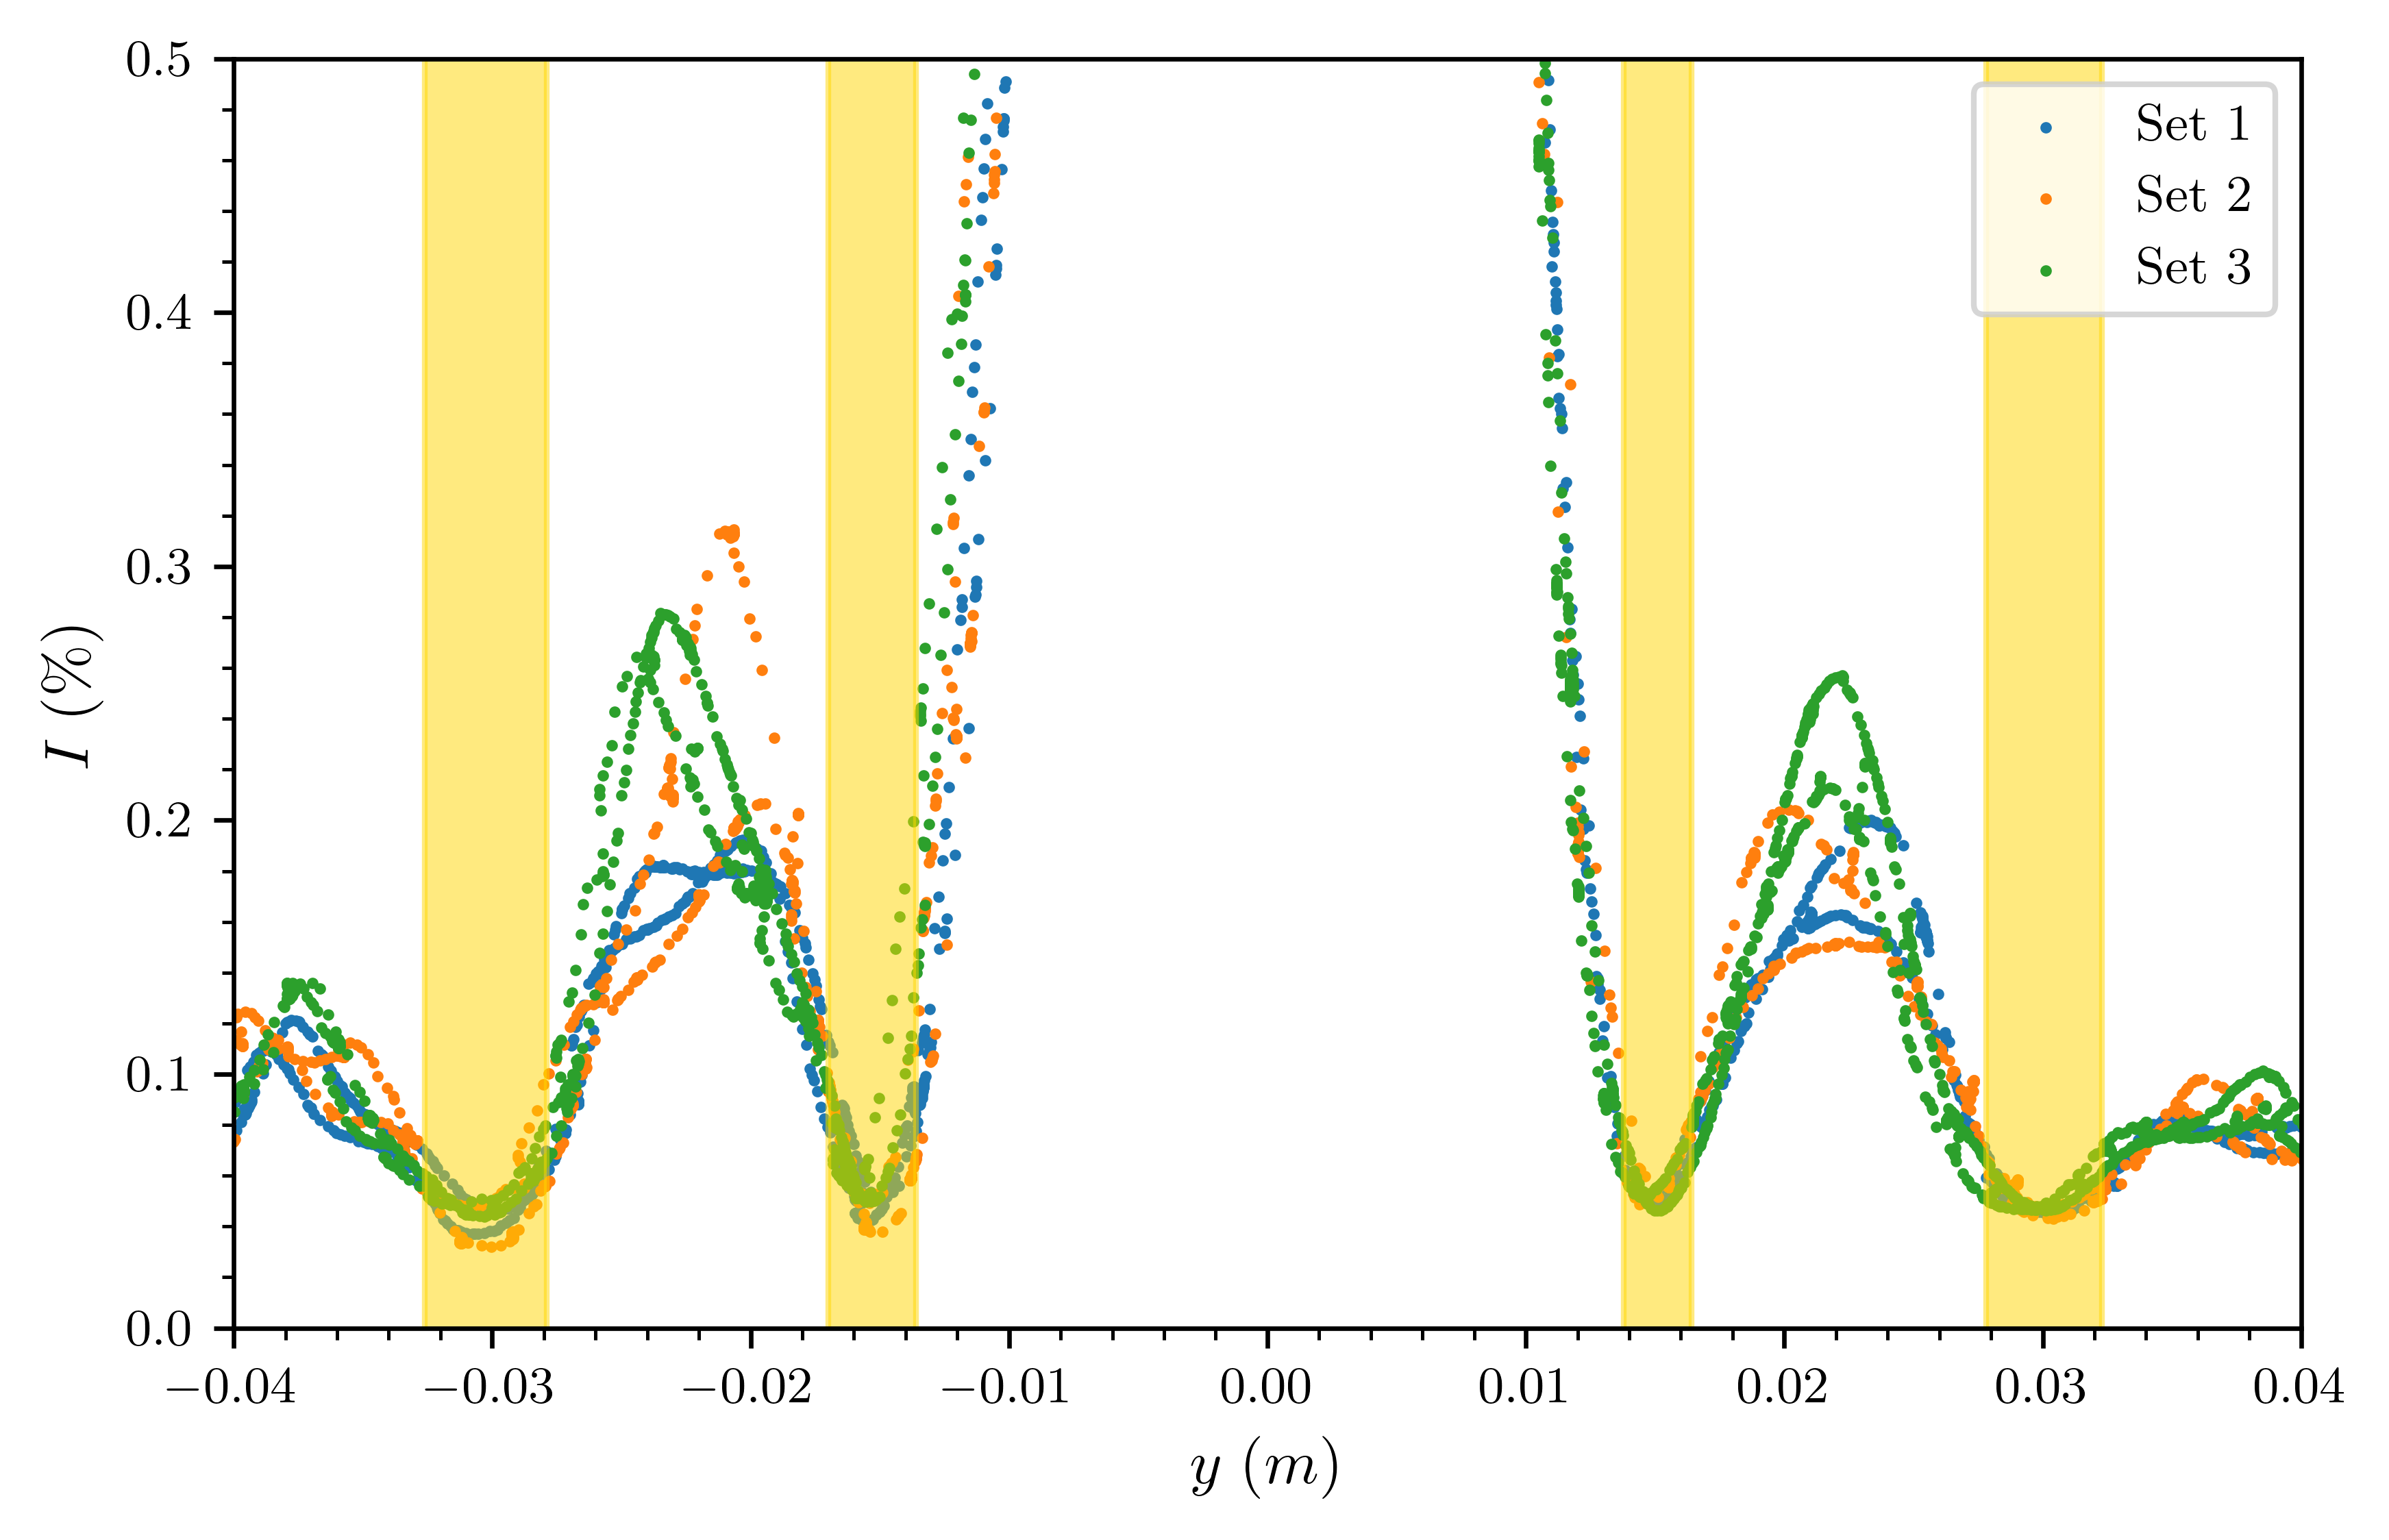
\includegraphics{min_0.04.png}
    \caption{Intensità luminosa $I$ in funzione della posizione $y$ del sensore (in metri) per la fenditura a \qty{0.04}{\mm}. In figura sono segnati i minimi ricavati graficamente con i relativi errori. È possibile notare come i picchi laterali presentino varie deformazioni da cui non è tuttavia possibile individuare un segnale sovrapposto come nel caso della fenditura da \qty{0.02}{\mm}.} % todo: trovare una giustificazione per i picchi laterali
    \label{fig:minimi 0.04}
\end{figure}

\begin{table}[ht!]
    \centering
    \caption{Posizione dei minimi, ottenuta graficamente dalla \autoref{fig:minimi 0.04}, riportata di fianco al proprio indice $m$ ed al valore $a$ (in $\si{\mm}$) stimato seguendo la relazione esposta in \autoref{eq:y=0 values}. Il valore di $a$ derivato da ciascun minimo è stato ricavato ponendo $\lambda = \qty{650}{\nm}$ ed $L = \qty{98.5+-0.1}{\cm}$, per il calcolo dell'errore di $a$ è stato considerato solo quello di $y$ in quanto l'errore su $L$ è trascurabile.}
    \import{../tables/}{mins_0.04.tex}
    \label{tab:minimi 0.04}
\end{table}

Intersecando le barre d'errore dei valori ottenuti si ha $a_g = \qty{0.043+-0.003}{\mm}$ che risulta appena compatibile con il valore teorico.

% Prendendo in considerazione la somma delle barre d'errore dei valori ottenuti $a = \qty{0.043+-0.004}{\mm}$.

% Facendo una media pesata dei valori ottenuti si ha $a = \qty{0.0424+-0.0012}{\mm}$. %? media o intersezione

\newpage

Successivamente si è proceduto con il fit utilizzando l'\autoref{eq:fit} e ottenendo un valore della fenditura $a_f = \qty{0.044+-0.005}{\mm}$. Il grafico del fit è riportato in \autoref{fig:fit 0.04}.

\begin{figure}[ht!]
    \centering
    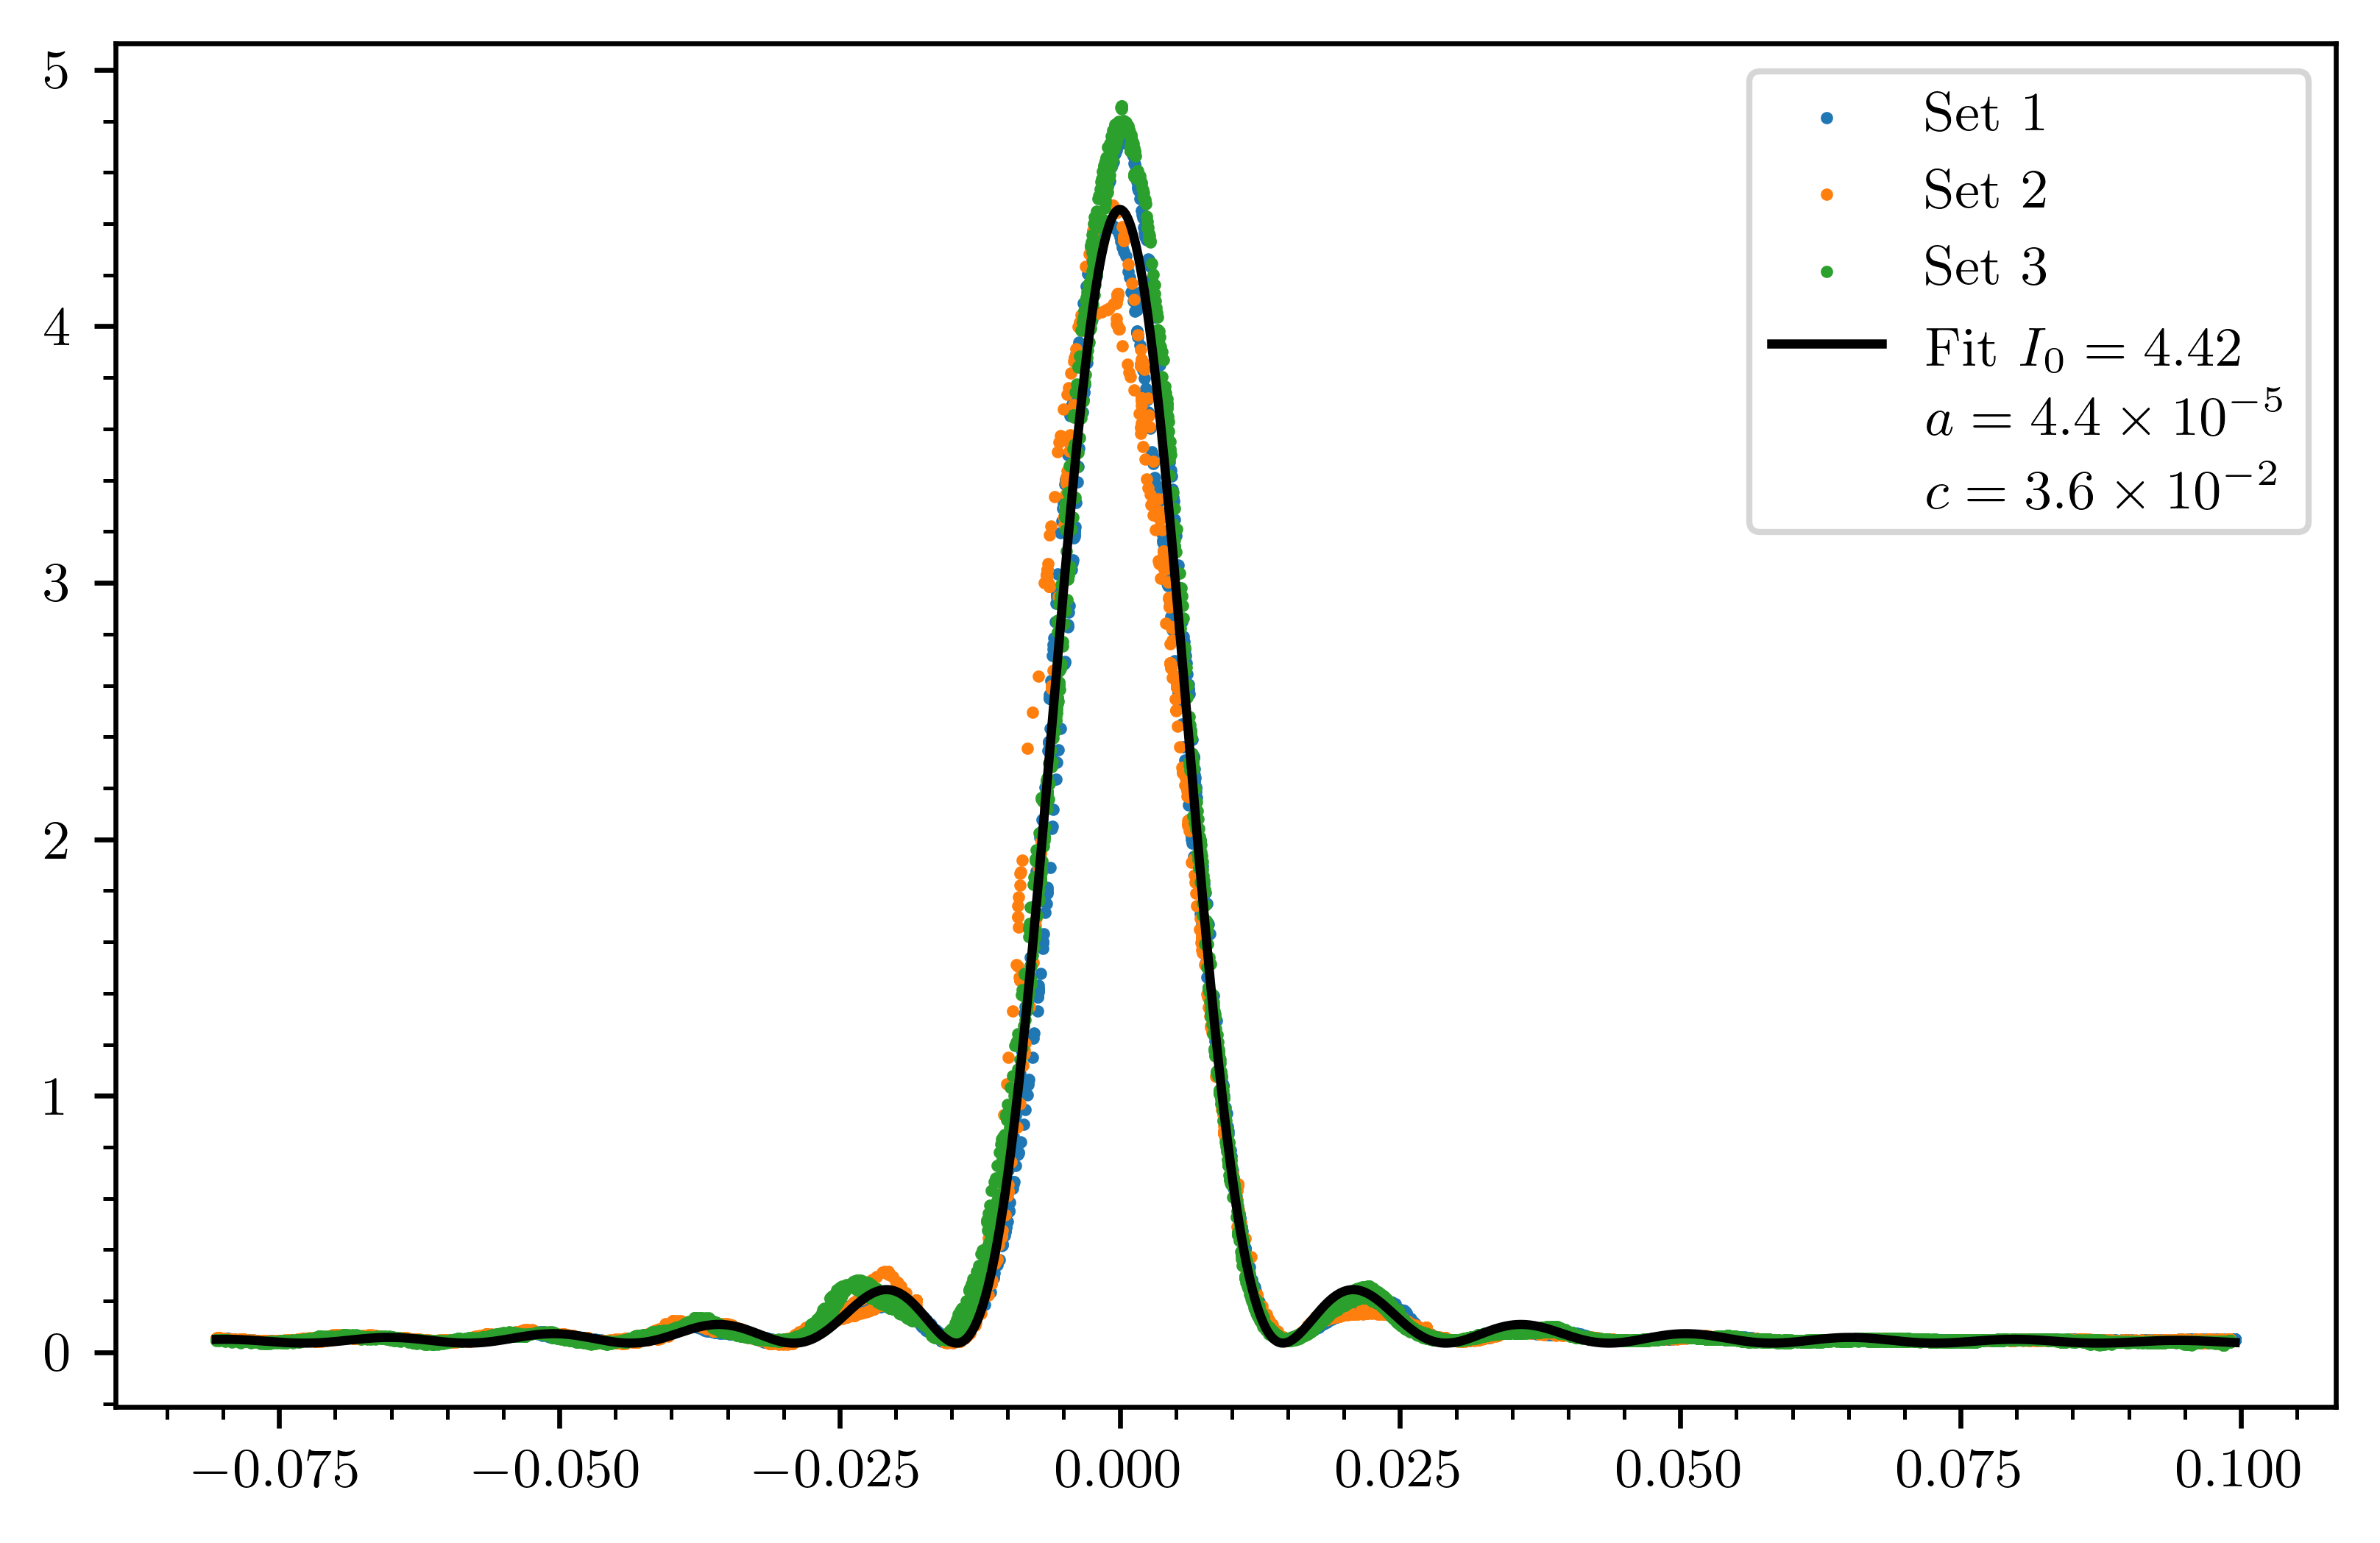
\includegraphics{fit_0.04.png}
    \caption{Intensità luminosa $I$ in funzione della posizione $y$ del sensore (in metri) per la fenditura a $\qty{0.04}{\mm}$. In figura è riportato il fit fatto utilizzando l'\autoref{eq:fit}. I valori dei parametri ottenuti sono $I_{0} = \num{4.42+-0.4}$, $a = \qty{0.044+-0.005}{\mm}$ e $c = \num{3.60+-0.02}$. }
    \label{fig:fit 0.04}
\end{figure}

Entrambi $a_g$ e $a_f$ risultano compatibili con il valore teorico di $a = \qty{0.04}{\mm}$.

Per confrontare le misure ottenute con diverse aperture del sensore si è scelto di utilizzare il set $3$ delle misure con apertura $\qty{1.5}{\mm}$, in quanto presenta una alta densità di misure lungo il picco e una variazione trascurabile dell'intensità massima. Dopo aver scalato le intensità dei set utilizzati in modo che il valore massimo di $I$ risultasse pari ad $1$ per tutti i set, essi sono stati riportati sovrapposti in \autoref{fig:sensore 0.04}, tuttavia non è stato possibile evidenziare alcuna correlazione tra l'ampiezza del sensore e la larghezza del picco centrale.

\begin{figure}[ht!]
    \centering
    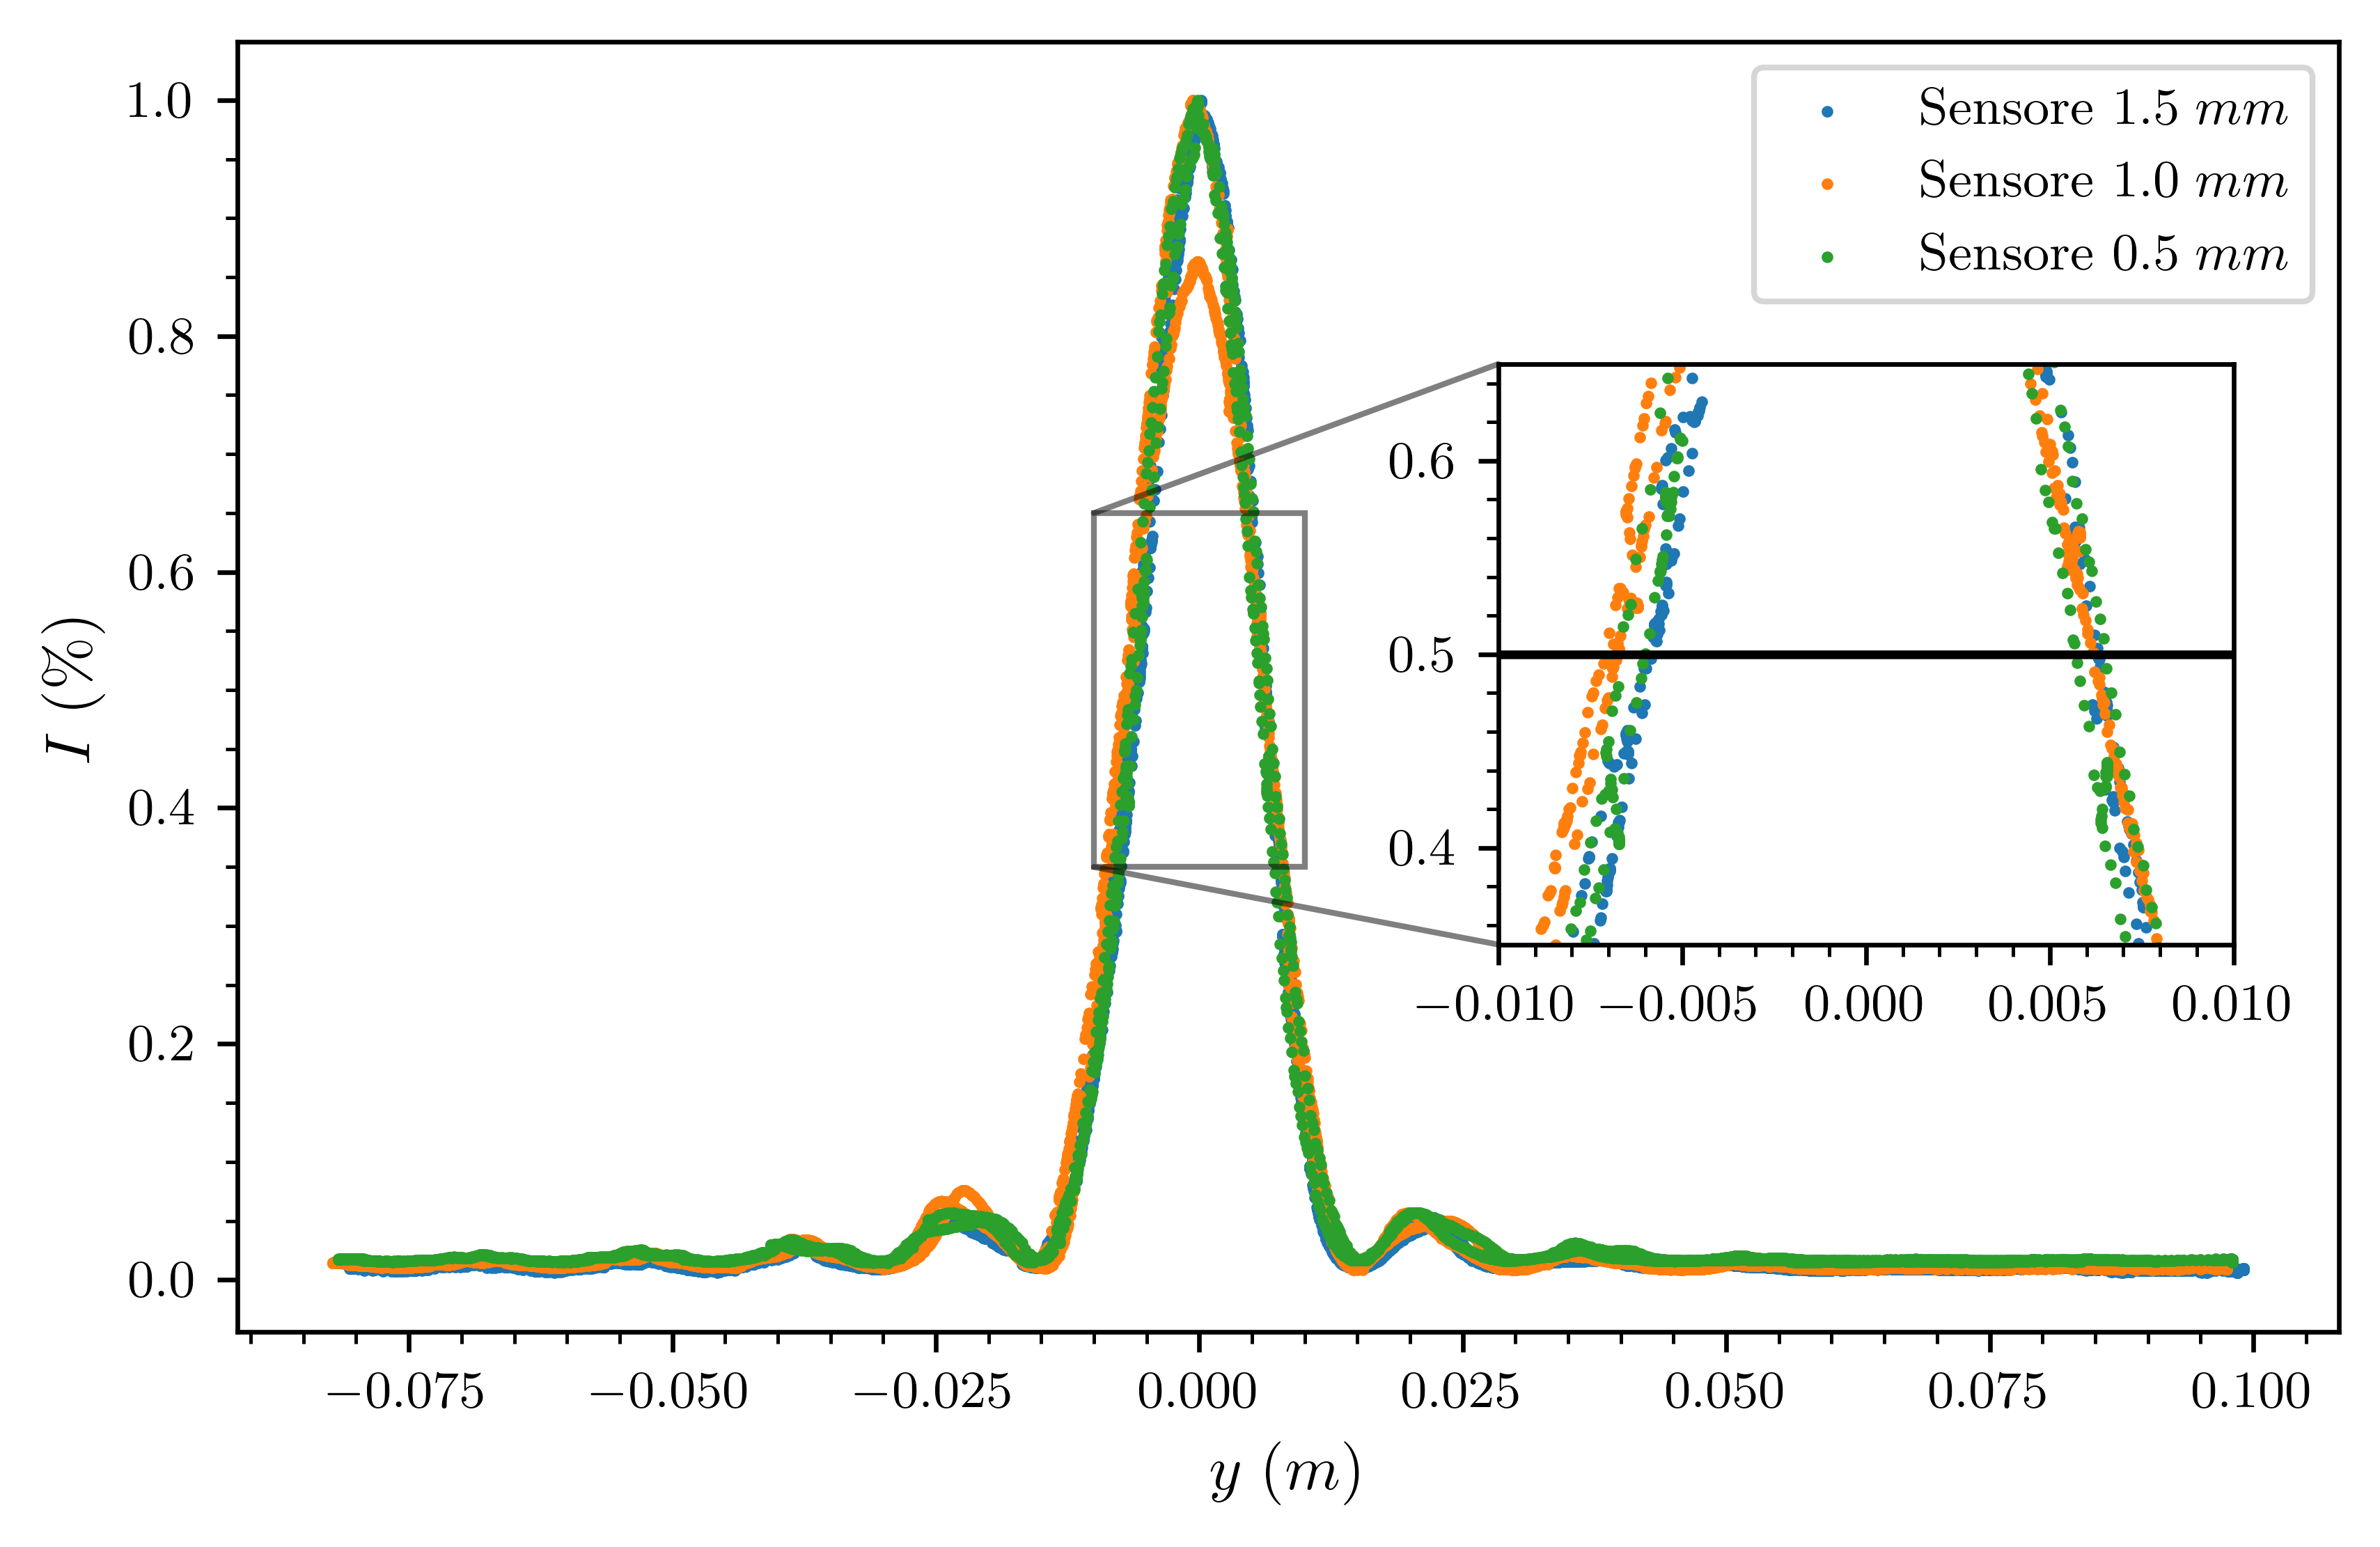
\includegraphics{sensor_0.04.png}
    \caption{Grafico dell'intensità luminosa relativa $I$ in funzione della posizione $y$ (in metri) per ciascuna delle due aperture del sensore.
    Tutti i set sono stati misurati con il fondoscala intermedio (\textit{lampadina}). I valori delle intensità sono stati scalati in modo che l'altezza del picco centrale fosse pari a $1$.
    Dato che la curva con apertura del sensore pari a \qty{1.5}{\mm} ha il picco più stretto delle altre, mentre quello con apertura pari a \qty{1.0}{\mm} risulta essere più ampio non è possibile evidenziare alcuna correlazione tra l'ampiezza del sensore e la larghezza del picco centrale.}
    \label{fig:sensore 0.04}
\end{figure}

\end{document}